\section{Literature Review: Oct 2023}
\sectionframe

\begin{frame}{Search Terms}
	\begin{itemize}
		\item transition metal phosphor sulfates OR FePS3 OR NiPS3 OR CrPS4 OR MnPS3
		\item spectroscopy of transition metal phosphor sulfates OR FePS3 OR NiPS3 OR CrPS4 for magnetic field
		\item magnetic order OR magnetic phase in semiconductor AND spectroscopy
		\item kerr OR moke OR Magnetic Circular Dichroism Spectroscopy
	\end{itemize}
\end{frame}

\begin{frame}{Magnetic Structure and Metamagnetic Transitions in the van der Waals Antiferromagnet \textbf{CrPS4} - 1/3}
	\begin{columns}
		\column{.5\textwidth}
		\fullgraphic{phase_diagram.png}
		\small
		\par{A-AFM:} $\vec{m} \parallel \vec{n}_\text{lattice}=\vec{c}$
		\par{C-AFM:} $\vec{m} \nparallel \vec{c}$ (canted)
		\column{.2\textwidth}
		\fullgraphic{image1.png}
	\end{columns}

\end{frame}

\begin{frame}{Magnetic Structure and Metamagnetic Transitions in the van der Waals Antiferromagnet CrPS4 - 2/3}
	\begin{columns}
		\column{0.6\textwidth}
		\fullgraphic{image3.png}
		\column{.15\textwidth}
		\fullgraphic{image1.png}
		\column{.3\textwidth}
		$\theta=\measuredangle(\vec c, \vec H)$ is important!
		\\\vspace{1em}
		$\chi(B\approx 0, T\approx 0)\approx 0$ is a property of AFM?
		\\ \vspace{1em}
		A-AFM -- C-AFM transition based on $\dv{M}{H}$ (b)
	\end{columns}
\end{frame}

\begin{frame}{Magnetic Structure and Metamagnetic Transitions in the van der Waals Antiferromagnet CrPS4 - 3/3 Torque}
	\begin{columns}
		\column{0.7\textwidth}
		\fullgraphic{image4.png}
		\column{.3\textwidth}
		C-AFM -- FM transition based on $\dv[2]{\text{Torque}}{H}$ (a,b)
	\end{columns}
\end{frame}

\begin{frame}{Magnetism in the layered transition-metal thiophosphates MPS3}
	\begin{columns}
		\column{0.6\textwidth}
		\fullgraphic{image10.png}
	\column{.4\textwidth}
		Heisenberg model $\Rightarrow$ different splitting for different $\measuredangle(\vec H, \vec n)$
	\end{columns}
\end{frame}

\begin{frame}{Magnetization Study of the AFM-FM Coexistence in the Manganite System Pr$_\text{0.5}$Ca$_\text{0.5-x}$Sr$_\text{x}$MnO$_3$}
	Coexistence of AFM in the bulk interior and FM at the surface\\
	$\Rightarrow$ Different behaviour in Kerr (surface) and Faraday?

	\vspace{1em}
	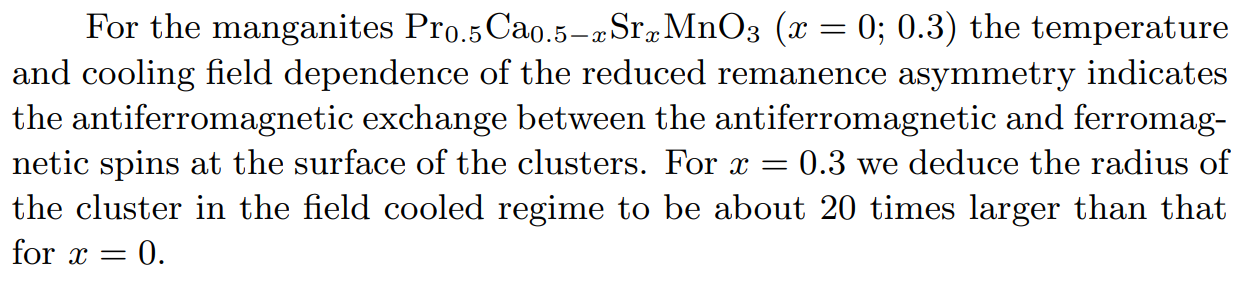
\includegraphics[width=\textwidth]{image5.png}
\end{frame}

\begin{frame}
	\textcolor{seeblau}{Field-dependent magneto-optical Kerr effect spectroscopy applied to the magnetic component diagnosis of a rubrene/Ni system}
	\begin{columns}
		\column{.5\textwidth}
		\fullgraphic{image6.png}
		\column{.4\textwidth}
		\small
		Rubrene: organic semiconductor
		\\ \vspace{1em}
		\fullgraphic{image7.png}
	\end{columns}
\end{frame}

\begin{frame}{Magnetic Order and Symmetry in the 2D Semiconductor CrSBr}
	\begin{columns}
		\column{0.7\textwidth}
		\fullgraphic{image9.png}
	\end{columns}
\end{frame}